\documentclass[border=5pt]{standalone}
    \usepackage{tikz}
    \usetikzlibrary{arrows.meta}

    \begin{document}
    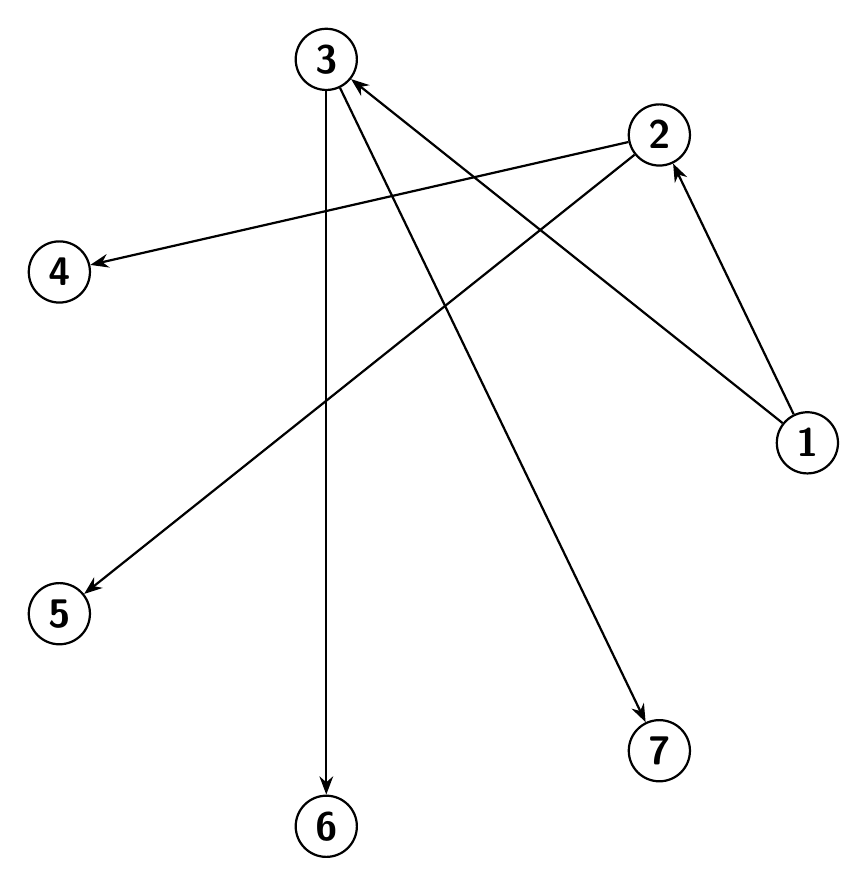
\begin{tikzpicture}[->, >=Stealth, auto, node distance=2.5cm, thick,
        main node/.style={circle, draw, font=\sffamily\Large\bfseries}]

        % Wierzcho�ki
    \node[main node] (1) at (5.00,0.00) {1};
    \node[main node] (2) at (3.12,3.91) {2};
    \node[main node] (3) at (-1.11,4.87) {3};
    \node[main node] (4) at (-4.50,2.17) {4};
    \node[main node] (5) at (-4.50,-2.17) {5};
    \node[main node] (6) at (-1.11,-4.87) {6};
    \node[main node] (7) at (3.12,-3.91) {7};

    % Kraw�dzie
    \path (1) edge[] (2);
    \path (1) edge[] (3);
    \path (2) edge[] (4);
    \path (2) edge[] (5);
    \path (3) edge[] (6);
    \path (3) edge[] (7);
\end{tikzpicture}
    \end{document}